\subsection{Những khái niệm cơ bản về đồ thị}
\subsubsection{Khái niệm đồ thị}
Một đồ thị là một cấu trúc rời rạc gồm tập hợp các đỉnh và các cạnh nối giữa các đỉnh đó. Có thể mô tả đồ thị theo cách hình thức như sau:\\
\centerline{\textbf{G = (V,E)}}
tức là đồ thị \textbf{G} có tập các đỉnh là \textbf{V}, tập các cạnh là \textbf{E}. Có thể hiểu \textbf{E} là tập hợp các cặp (u, v) với u và v là hai đỉnh thuộc V.\\
Tập các đỉnh V của đồ thị G có thể là vô hạn. Một đồ thị có tập đỉnh vô hạn hoặc vô số cạnh được gọi là đồ thị vô hạn, và khi so sánh, đồ thị có tập đỉnh hữu hạn và tập hợp cạnh hữu hạn được gọi là đồ thị hữu hạn
\begin{figure}[H] % places figure environment here   
    \centering % Centers Graphic
    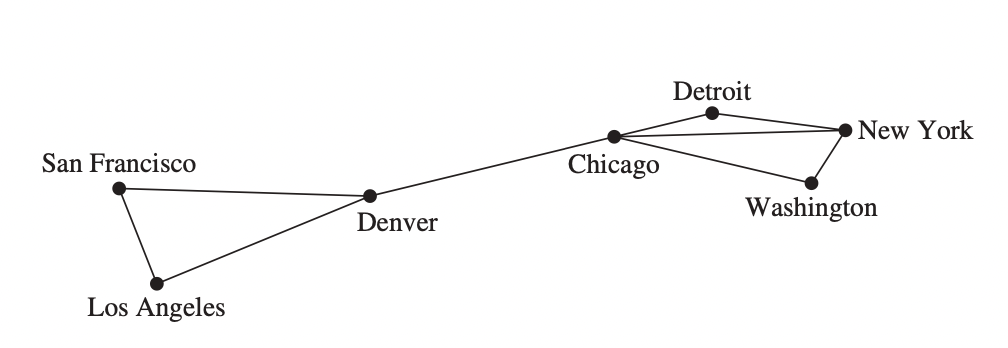
\includegraphics[width=0.6\textwidth]{assets/computer_network.png} 
    \caption{Mạng máy tính} % Creates caption underneath graph
    \label{fig:gr_1.1.1}
\end{figure}
Bây giờ, giả sử rằng một mạng được tạo thành từ các trung tâm dữ liệu và các liên kết giao tiếp giữa các máy tính. Chúng ta có thể biểu diễn vị trí của mỗi trung tâm dữ liệu bằng một điểm và mỗi liên kết truyền thông liên kết bằng một đoạn thẳng, như thể hiện trong Hình 1.\\
\subsubsection{Phân loại đồ thị}
Có thể phân loại đồ thị G theo tính chất các tập cạnh như sau:\\
\begin{figure}[H] % places figure environment here   
    \centering % Centers Graphic
    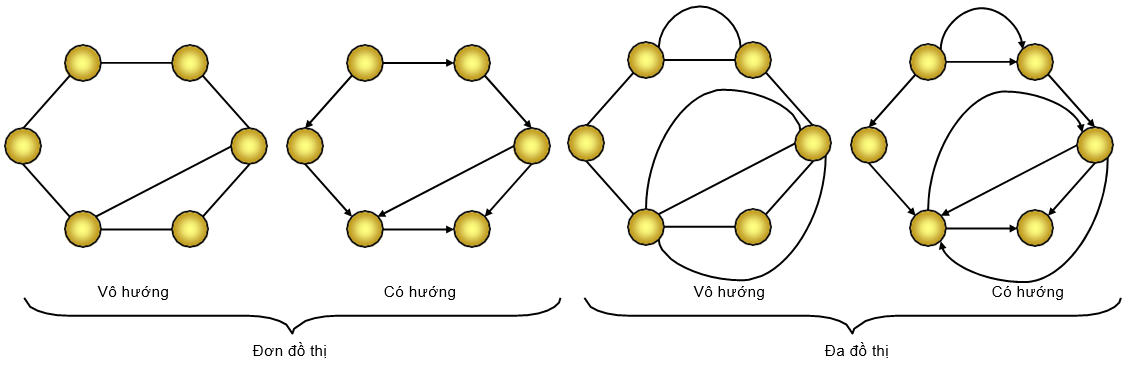
\includegraphics[width=0.8\textwidth]{assets/phanloaidothi.png} 
    \caption{Phân loại đồ thị} % Creates caption underneath graph
    \label{fig:gr_1.2.2}
\end{figure}
\begin{enumerate}
\item{\textbf{Đơn đồ thị}} \\
    G được gọi là đơn đồ thị nếu như giữa hai đỉnh (u, v) của V có nhiều nhất một cạnh trong E nối từ u tới v.\\
    Như Hình 1 là một đơn đồ thị. Mạng máy tính này có thể được mô hình hóa bằng cách sử dụng một đồ thị trong đó các đỉnh của đồ thị đại diện cho các trung tâm dữ liệu và các cạnh đại diện cho các liên kết truyền thông. Lưu ý rằng mỗi cạnh của đồ thị đại diện cho mạng máy tính này kết nối hai đỉnh khác nhau. Có nghĩa là, không có cạnh nào kết nối một đỉnh với chính nó. Hơn nữa, không có hai cạnh khác nhau nối cùng một cặp đỉnh.
\item{\textbf{Đa đồ thị}} \\
    G được gọi là đa đồ thị nếu như giữa hai đỉnh (u, v) của V có thể có nhiều hơn 1 cạnh nối trong E nối từ u tới v. Hiển nhiên đơn đồ thị cũng là đa đồ thị.
    \begin{figure}[H] % places figure environment here   
        \centering % Centers Graphic
        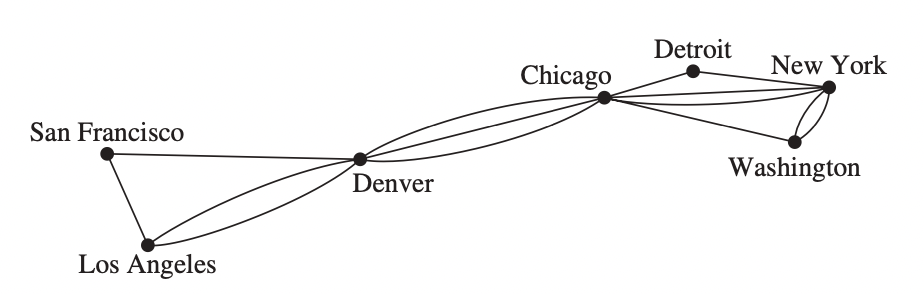
\includegraphics[width=0.6\textwidth]{assets/da_dothi.png} 
        \caption{Đa đồ thị} % Creates caption underneath graph
        \label{fig:gr_1.1.3}
    \end{figure}
    Một mạng máy tính có thể chứa nhiều liên kết giữa các trung tâm dữ liệu, như trong Hình 3. Để mô hình hóa các mạng như vậy, chúng ta cần các đồ thị có nhiều hơn một cạnh nối cùng một cặp đỉnh. Các đồ thị có thể có nhiều cạnh nối các đỉnh giống nhau được gọi là đồ thị đa phương. Khi có m cạnh khác nhau liên kết với cùng một cặp đỉnh không có thứ tự {u, v}, ta cũng nói rằng {u, v} là một cạnh bội số m. Tức là, chúng ta có thể coi tập hợp các cạnh này là m bản sao khác nhau của một cạnh {u, v}.
\item{\textbf{Đồ thị vô hướng}} \\
    G được gọi là đồ thị vô hướng (undirected graph) nếu như các cạnh trong E là không định hướng, tức là cạnh (u, v) là cạnh hai chiều.\\
\item{\textbf{Đồ thị có hướng}} \\
    G được gọi là đồ thị có hướng (directed graph) nếu như các cạnh trong E là có định hướng.\\
    Khi chúng ta mô tả một đồ thị có hướng bằng một bản vẽ đường thẳng, chúng ta sử dụng một mũi tên chỉ từ u đến v để chỉ ra hướng của một cạnh bắt đầu tại u và kết thúc tại v. Một biểu đồ có hướng có thể chứa các vòng lặp và nó có thể chứa nhiều cạnh có hướng bắt đầu và kết thúc ở cùng một đỉnh. Một đồ thị có hướng cũng có thể chứa các cạnh có hướng nối các đỉnh u và v theo cả hai hướng; nghĩa là, khi một đồ thị chứa một cạnh từ u đến v, nó cũng có thể chứa một hoặc nhiều cạnh từ v đến u.\\
    Khi một đồ thị có hướng không có vòng lặp và không có nhiều cạnh có hướng, nó được gọi là \textbf{đồ thị có hướng đơn giản}. Bởi vì một đồ thị có hướng đơn giản có nhiều nhất một cạnh liên kết với mỗi cặp đỉnh có thứ tự (u, v), chúng ta gọi (u, v) là một cạnh nếu có một cạnh liên kết với nó trong đồ thị.\\
    Các đồ thị có hướng có thể có nhiều cạnh có hướng từ một đỉnh đến một đỉnh thứ hai (có thể giống nhau) được sử dụng để mô hình hóa các mạng như vậy. Những đồ thị như vậy là \textbf{đồ thị đa hướng}. Khi có m cạnh có hướng, mỗi cạnh liên kết với một cặp đỉnh có thứ tự (u, v), chúng ta nói rằng (u, v) là một cạnh của m.\\
    \begin{figure}[H] % places figure environment here   
        \centering % Centers Graphic
        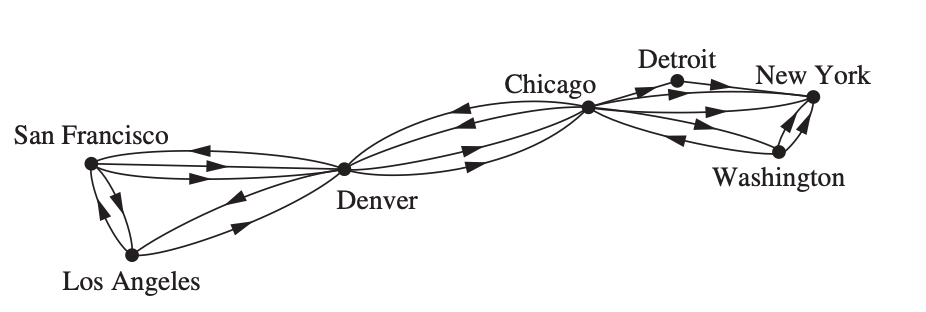
\includegraphics[width=0.6\textwidth]{assets/dothi_dahuong.png} 
        \caption{Đồ thị đa hướng} % Creates caption underneath graph
        \label{fig:gr_1.1.4}
    \end{figure}
\end{enumerate}
\subsubsection{Đường đi và chu trình}
Gọi n là một số nguyên không âm và G là một đồ thị vô hướng. 
Đường đi có độ dài n từ u đến v trong G là dãy gồm n cạnh $e_1, ..., e_n$ của G mà trong đó tồn tại dãy $x_0 = u, x_1, ..., x_{n-1}, x_n = v$ thuộc các đỉnh sao cho $e_i$, với i = 1, ..., n, các điểm cuối $x_{i-1}$ và $x_i$. 
Khi đồ thị đơn giản, ta biểu thị đường đi này bằng dãy đỉnh $x_0, x_1, ..., x_n$ (vì liệt kê các đỉnh này xác định duy nhất đường đi).\\
Đường đi là \textbf{một chu trình} nếu nó bắt đầu và kết thúc tại cùng một đỉnh, nghĩa là, nếu u = v, và có độ dài lớn hơn 0. Đường đi hoặc chu trình được cho là đi qua các đỉnh $x_1, x_2, ..., x_{n-1}$ hoặc đi qua các cạnh $e_1, ..., e_n$. Một đường đi hoặc chu trình sẽ đơn giản nếu nó không chứa cùng một cạnh nhiều hơn một lần.\\
Đường đi được gọi là đường đi đơn giản (simple path) nếu tất cả các đỉnh trên đường đi đó đều phân biệt. Đường đi được gọi là đường đi đơn nếu như không có cạnh nào trên đường đi đó đi qua hơn một lần.\\
Chu trình gọi là chu trình đơn giản (simple circuit) nếu như {$x_1, x_2,..., x_k$}v đôi một khác nhau. Chu trình mà trong đó không có cạnh nào đi qua hơn một lần được gọi là chu trình đơn.\\
\textit{Ví dụ:}\\
\begin{figure}[H] % places figure environment here   
    \centering % Centers Graphic
    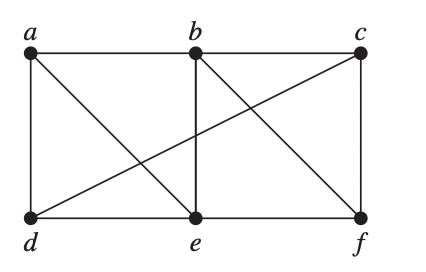
\includegraphics[width=0.5\textwidth]{assets/duongdi_dongian.png} 
    \caption{Đơn đồ thị} % Creates caption underneath graph
\end{figure}
Trong đồ thị trên, a, d, c, f, e là một đường đi đơn giản có độ dài 4, bởi vì {a, d}, {d, c}, {c, f} và {f, e } là tất cả các cạnh. Tuy nhiên, d, e, c, a không phải là đường đi, vì {e, c} không phải là cạnh. Lưu ý rằng b, c, f, e, b là một chu trình có độ dài 4 vì {b, c}, {c, f}, {f, e} và {e, b} là các cạnh và đường đi này bắt đầu và kết thúc ở b. Đường đi a, b, e, d, a, b có độ dài 5 không phải là đường đi đơn vì nó chứa cạnh {a, b} hai lần.
